\graphicspath{ {./images/} }
\section{Operation of the System}

The architecture of PECAN comprises a search engine message store, and web-server back-end, and a several add-ons that provide the functionality for running user studies and batch-style evaluation for the task of search for conversations. PECAN is made for bring-your-own-data: it provides the tools to search, present, and perform experiments on your data, but it does not provide a means to scraping chat messages. As such, an overview of the fields that are required to be indexed for the basic functioning of PECAN are presented in Table~\ref{table:fields}. We have chosen these fields as, in our opinion, they are the minimum required fields that almost all chat messaging systems today would use.

\begin{table}
\centering
\begin{tabular}{ll}
	\hline
	Field     & Description                                        \\ \hline
	Text      & The textual content of a message.                  \\
	Timestamp & The time and date that a message was sent.         \\
	User      & The user (or user identifier) that sent a message. \\
	Type      & The type of message that is sent.                  \\
	Channel   & Where a message was sent.                          \\ \hline
\end{tabular}
\caption{Necessary fields that must be included in the message index for the correct operation of PECAN. The purpose of the \textit{Type} field is to visually present messages in different ways, e.g., quoted messages. The \textit{Channel} field specifies the `location' the message was sent in a chat system, e.g., the public/private spaces of services such as Slack or Discord, or the groups or direct messages of services such as Signal or Whatsapp (note that services such as Slack and Discord also have direct messages).}
\label{table:fields}
\end{table}

\subsection{Searching for Conversations}

%\todo{1st priority: for @kq: use images to describe how a user uses the system. each image has a caption, in the text expand upon the caption. give a "fake" case study, the user first enters a query, then they look through conversations, then they do blah... etc.}
We first present a small case study that demonstrates some of the user interfaces that are built into PECAN. The homepage (Figure~\ref{fig:homepage}) of PECAN shows statistics about the number of messages that are indexed and several recent messages that have been indexed. One thing to note immediately is that it is possible for PECAN to (optionally) apply the same security considerations as the system that was originally used to send the messages. This allows private messages within a chat system to remain private. We achieve this by providing a pluggable authentication system.~\footnote{For more information about this, please refer to the GitHub repository.} Within the homepage, users may enter queries and filter their query to certain time periods, channels, and other users (depending on the original chat system). PECAN can also be configured to record query logs and fine-grained user interactions with the system, for improving searching for conversations effectiveness and for studying user behaviour in a user study setting.

Once users issue a query to PECAN, they are presented with a conversations results page (CORP), as presented in Figure~\ref{fig:searching}. On this page, users can explore conversations that are relevant to their query. Conversations are ranked according to their relevance to a given query. We describe our approach to scoring conversations in Section~\ref{sec:conv-scoring}. We choose to select five messages before and after a retrieved message to form a conversation. Note that this may result in some conversations with overlapping messages. To address this, we propose to aggregate conversations with overlapping messages. As a result, the CORP may contain conversations with more than ten messages. Our approach to aggregating conversations is described in Section~\ref{sec:conv-agg}.

Finally, each conversation in the CORP can be further explored by viewing messages that occur before or after a conversation. Each conversation in the CORP contains buttons to view messages that occur before or after a conversation. Users are able to cycle through more messages indefinitely in order to fulfil their information need. The interface that users can use to explore these messages is presented in Figure~\ref{fig:traversing}.

\begin{figure}
	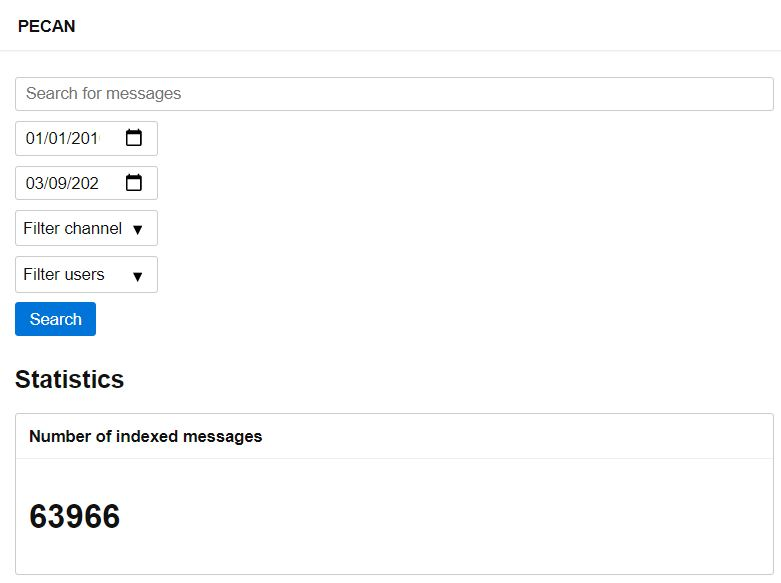
\includegraphics[width=\linewidth]{homepage}
	\caption{The homepage of PECAN. Here, users can enter their search query and apply any search filters to refine their search. Statistics about the number of messages that are indexed are also shown, alongside several recently indexed messages.}
	\label{fig:homepage}
\end{figure}

\begin{figure}
	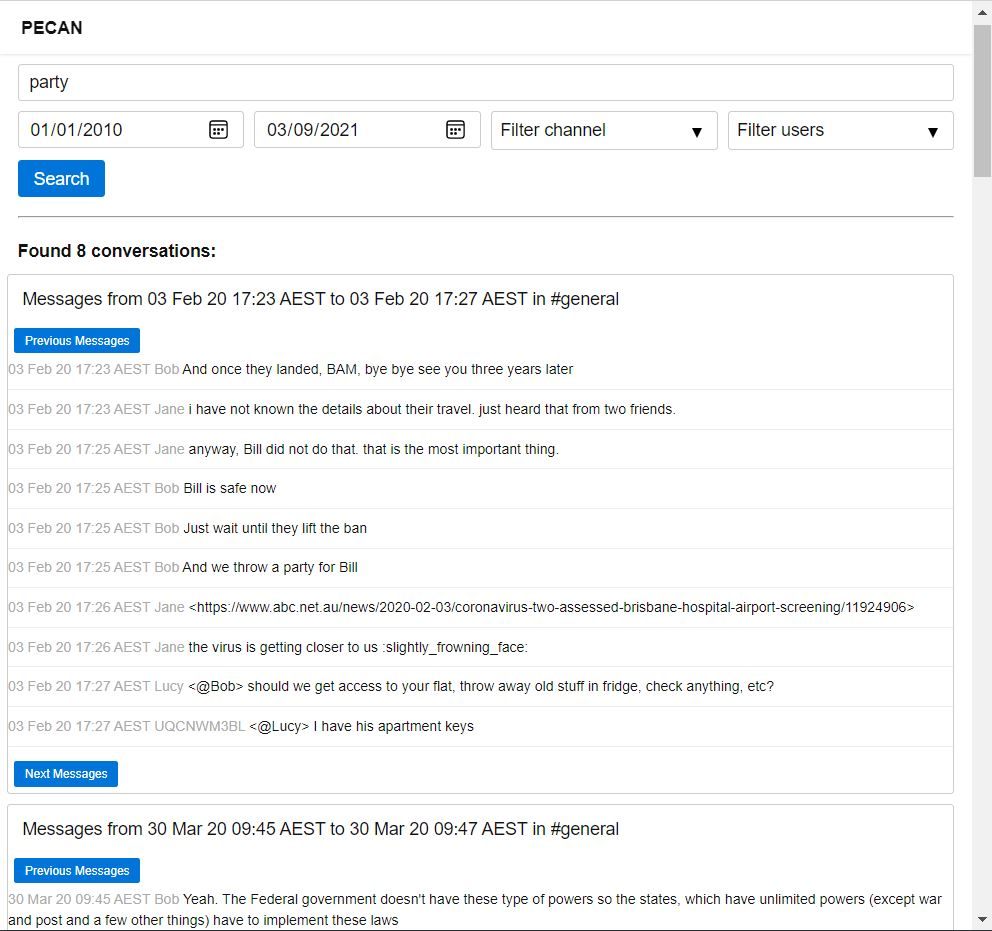
\includegraphics[width=\linewidth]{searching}
	\caption{The CORP page of a response to an example query `party'. Each conversation is ranked in terms of relevance to the input query, similar to contemporary SERPs. Conversations can be explored further by interacting with the `Previous Messages' and `Next Messages' buttons at the start and end of each conversation.}
	\label{fig:searching}
\end{figure}

\begin{figure}
	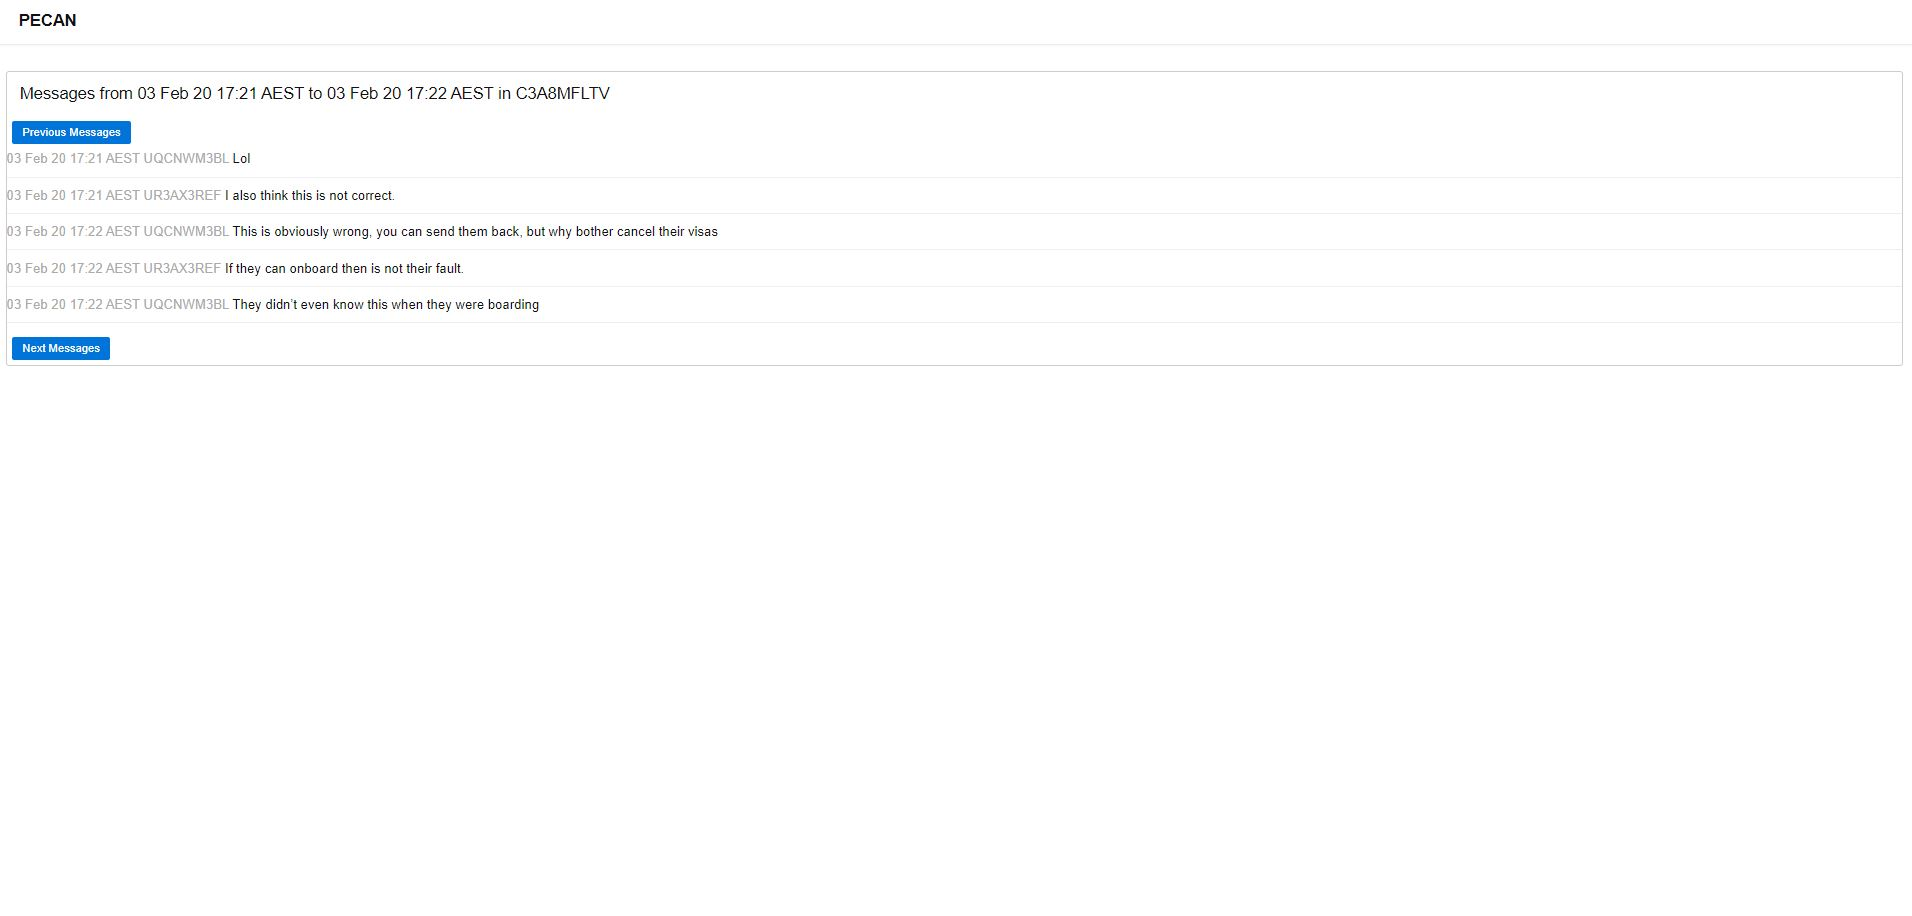
\includegraphics[width=\linewidth]{traversing}
	\caption{The conversation exploration page that users are presented with after clicking one of the `Previous Messages' or `Next Messages' buttons at the start and end of each conversation on the CORP. Users can continue to load more messages in the conversation indefinitely.}
	\label{fig:traversing}
\end{figure}


\subsection{System Implementation}

PECAN is implemented using the Go programming language. Go was chosen as it has been demonstrated to be an efficient server programming language. This is important as there may considerable overhead in more advanced algorithms than we have proposed that need to be executed at retrieval time (e.g., more complex conversation aggregation or scoring algorithms). For the underlying message storage engine, we use Elasticsearch 7.x. Elasticsearch is a highly scaleable search engine that is capable of ingesting and retrieving documents (in our case messages) in real time.

Of the searching for conversation related research tasks that we raise in Section~\ref{sec:importance}, we have provided baseline implementations of two: conversation aggregation and conversation scoring. The following two sections provide a description of how we implement these methods in PECAN. These implementations are part of a pluggable system, where new implementations are designed to be easy to add and extend. Please refer to the GitHub repository for details on how to implement new methods.

\subsubsection{Conversation Aggregation}
\label{sec:conv-agg}

There are many ways to retrieve conversations instead of messages, for example, one could decide to group messages together based on time, topicality, among others. The default behaviour we provide in PECAN is to aggregate messages into conversations based on the time messages were sent. A high-level overview of this algorithm is provided in Algorithm~\ref{algo:overview}. To form conversations, we first retrieve individual messages given a query. Next, we retrieve the five messages that were sent before and after the original message (including the original message). This is a fast operation within Elasticsearch, and can be done at retrieval time. All ten messages are then combined into a single conversation. One implementation detail we note is that for chat systems that have multiple `channels', we do not merge messages from different channels. This is because we believe that a conversation is tied to the context with which it occurred.

Following the creation of the conversations, we proceed to merge conversations that contain overlapping messages. This process is detailed in Algorithm~\ref{algo:overview}.



\begin{algorithm}
	\SetAlgoLined
	\caption{High-level overview of how conversations are retrieved, scored, and ranked given a query.}
	\label{algo:overview}
	\SetKwInOut{Input}{inputs}
	\SetKwInOut{Output}{output}
	\Input{search query $q$}
	\Output{list of conversations $C$}
	Initialise messages $M$ as the result of executing $q$\\
	Initialise $C\gets\emptyset$\\ 
	\ForEach{$m\in M$}{
		Add to $C$ the list of $k$ surrounding messages of $m$\\
	}
    Merge any overlapping $c\in C$ using Algorithm~\ref{algo:merge}\\
	\Return{C}\end{algorithm}
		
\begin{algorithm}
	\SetAlgoLined
	\caption{Merge Conversations \todo{@kq: simplify this}}
	\label{algo:merge}
	\SetKwInOut{Input}{inputs}
	\SetKwInOut{Output}{output}
	\SetKwProg{MergeConversations}{MergeConversations}{}{}
	\MergeConversations{$(conversations)$}{
		\Input{$conversations$}
		\Output{$C$}
		$mergedConvs \gets []$\\
		$H \gets HashMap$\\
		\ForEach{$conversation \in conversations$}{
			$index \gets H.get(conversation[0].Channel)$\\
			\If{$index \neq null$ and $conversation$ overlap with $mergedConvs[index]$}{
				\ForEach{$message \in conversation$}{
					\If{$message$ is older than $mergedConvs[index]$}{
						$mergedConvs[index].append(message)$
					}
					\ElseIf{$message.Score>0$}{
						\ForEach{$keyMessage \in mergedConvs[index]$}{
							\If{$keyMessage$ and $message$ have same timestamp and content}{
								$keyMessage \gets message$
							}
						}
					}
				}
			}
			\Else{
				$mergedConvs.append(conversation)$
				$H[conversation[0].Channel] = len(C) -1$
			}
		}
		\Return{$mergedConvs$}
	}
\end{algorithm}		
		
\subsubsection{Conversation Scoring}
\label{sec:conv-scoring}

After merging conversations, we rank these conversations based on their scores. Our conversation scoring method exploits the fact that individual messages are scored at retrieval time (i.e., line 1 in Algorithm~\ref{algo:overview}). By default, each conversation inherits the score assigned to the original message that formed the conversation. However, when a conversation is composed by merging two conversations together, we sum the scores of the two messages that overlap.


\subsection{Add-ons}

PECAN is designed to be a flexible research tool for conducting experiments involving the task of searching for conversations. As such, we provide two add-ons that cover many of the types of research that we see others performing.

\subsubsection{Running a User Study}

In addition to the common use-case of searching for conversations, as any organisation or individual may want to use PECAN for, we also provide research-grade user study facilities in the form of an add-on. This add-on allows one to study aspects to searching for conversations such as user behaviour. In particular, the added functionality consists of:
\begin{description}[noitemsep, leftmargin=8pt]
\item[Query Logging] Queries that users issue to the system, and the filters that they apply can be logged directly to a file. 
\item[Interaction Logging] Fine-grained user interactions with the web browser, such as mouse movements or keyboard events, can be logged directly to a file.
\item[Screen Recording] Live screen recording of users interacting with the system, including their cursor, can be logged directly to a directory containing a series of images for each capture.
\end{description}

\subsubsection{Batch Evaluation}

Another add-on that we provide is the ability to run and evaluate batch-style evaluation for the task of searching for conversations. This add-on exposes a RESTful service where one may upload a set of queries and receive a TREC formatted run file as a response. In addition, one may specify an implementation of the research tasks listed in Section~\ref{sec:importance}. This could be to, for example, compare the effectiveness of two or more conversation scoring algorithms. 


%\subsection{Planned Features}
%The current implementation of the system is only a very fundamental template. In the future, we will add more features such as channel filtering, query suggestion, query logging and interaction logging. We will also bring up more research tasks based on this system, such as chat summerisation.
%
%\todo{4th priority: for @kq: channel filtering (in search time), filter by author, attachment search}




